%%===================================================================
%% Lecture 15 -- QCD + QED and Spontaneous Symmetry Breaking
%% 77609 -- Introduction to Elementary Particles
%% Date: 04/06/2026
%% Lecturer: Prof. Yonit Hochberg
%%===================================================================

\section{Lecture 15 -- QCD + QED and Spontaneous Symmetry Breaking}\label{sec:lec15}
\begin{center}
\begin{tabular}{ll}
  \textbf{Date:}\quad 04/06/2026 & \\
\end{tabular}
\end{center}
\hrule\vspace{1.5em}

%%------------------------------------------------------------------
\subsection{Overview}\label{subsec:lec15:overview}

Lecture~14 completed the construction of pure $\QCD$: local $SU(3)_c$, six Dirac quarks in the fundamental representation, eight gluons in the adjoint representation, and the characteristic non-Abelian gluon self-interactions. This lecture first adds electromagnetism and studies the theory
\[
  SU(3)_c\times U(1)_{\mathrm{EM}},
\]
which is a useful intermediate step toward the full Standard Model when weak interactions are neglected. The second and longer part of the lecture starts the next conceptual ingredient: spontaneous symmetry breaking. We begin with a global discrete $\mathbb Z_2$ symmetry, then move to a global continuous $U(1)$ symmetry, where the appearance of a massless Goldstone boson becomes visible.

\begin{enumerate}
  \item \textbf{$\QCD+\QED$}: field content, charges, covariant derivatives, kinetic terms, interactions, and accidental global symmetries.
  \item \textbf{Spontaneous symmetry breaking}: the Lagrangian is symmetric, but a chosen vacuum need not be.
  \item \textbf{Discrete example}: a real scalar with $\mathbb Z_2:\phi\to-\phi$ and two degenerate vacua.
  \item \textbf{Continuous example}: a complex scalar with global $U(1)$ symmetry, a Mexican-hat potential, one massive radial mode, and one massless angular mode.
  \item \textbf{Goldstone theorem}: every broken continuous global generator produces a massless boson.
\end{enumerate}

%%==================================================================
\subsection{Combining QCD with Electromagnetism}\label{subsec:lec15:qcd-qed}

\subsubsection*{Physical Motivation}

Pure $\QCD$ knows about color but not electric charge. Pure $\QED$ knows about electric charge but not color. Nature contains quarks carrying both quantum numbers: an up quark is a color triplet and has charge $+2/3$, while a down quark is a color triplet and has charge $-1/3$. Neglecting the weak interactions, the natural gauge group is therefore the direct product
\begin{equation}
  \boxed{\;G_{\QCD+\QED}=SU(3)_c\times U(1)_{\mathrm{EM}}\;}
  \label{eq:lec15:qcd_qed_gauge_group}
\end{equation}

\textit{Significance:} This product theory is the part of the Standard Model that already describes colored quarks, gluons, photons, and charged leptons before electroweak interactions are introduced.

\dfn[def:lec15:quark-fields-qcd-qed]{Quark Field Content under $SU(3)_c\times U(1)_{\mathrm{EM}}$}{
For generation index $i=1,2,3$, the chiral quark fields transform as
\begin{equation}
  \boxed{\;
  u_{Li}\sim(\mathbf3,+\tfrac23),\qquad
  u_{Ri}\sim(\mathbf3,+\tfrac23),\qquad
  d_{Li}\sim(\mathbf3,-\tfrac13),\qquad
  d_{Ri}\sim(\mathbf3,-\tfrac13)\; .}
  \label{eq:lec15:quark_representations}
\end{equation}
The first entry is the $SU(3)_c$ representation and the second entry is the electromagnetic charge $Q$ in units of the proton charge $e>0$.
}

\textit{Significance:} Electromagnetism splits the six quarks into two charge sectors, so up-type and down-type quarks can no longer be freely mixed by a single $U(6)$ flavor rotation.

Local gauge invariance forces us to include one gauge field for each generator of the gauge group. The $SU(3)_c$ factor has $3^2-1=8$ generators, so it gives eight gluons $G_\mu^a$, $a=1,\ldots,8$. The Abelian $U(1)_{\mathrm{EM}}$ factor has one generator, so it gives one photon $A_\mu$:
\begin{equation}
  G_\mu^a\sim(\mathbf8,0),\qquad A_\mu\sim(\mathbf1,0).
  \label{eq:lec15:gauge_bosons_representations}
\end{equation}
The photon is neutral under electromagnetism because an Abelian gauge boson carries no charge under its own group; the gluons are neutral under $U(1)_{\mathrm{EM}}$ because color and electric charge are independent gauge factors.

\subsubsection*{Mathematical Setup}

Let $\lambda^a$ be the Gell-Mann matrices, so the fundamental $SU(3)$ generators are $T^a=\lambda^a/2$. Let $g_s$ denote the strong coupling, $e$ the electromagnetic coupling, and $Q_f$ the electromagnetic charge of a field $f$. A color-triplet quark sees both gauge factors, so its covariant derivative is
\begin{equation}
  \boxed{\;D_\mu f
  =\left(\partial_\mu+\frac{i}{2}g_sG_\mu^a\lambda^a+i e Q_f A_\mu\right)f\; .}
  \label{eq:lec15:qcd_qed_covariant_derivative}
\end{equation}

\textit{Significance:} In a product gauge theory the covariant derivative is the sum of the gauge connections for each factor, with each term acting only through the representation and charge carried by the field.

For the four quark multiplets in Eq.~\eqref{eq:lec15:quark_representations}, the charge is
\begin{equation}
  Q_{u_L}=Q_{u_R}=+\frac23,\qquad
  Q_{d_L}=Q_{d_R}=-\frac13 .
  \label{eq:lec15:quark_charges}
\end{equation}
If a field were in a different $SU(3)$ representation, the matrices $\lambda^a/2$ in Eq.~\eqref{eq:lec15:qcd_qed_covariant_derivative} would be replaced by the generators of that representation.

The gauge-field strengths are
\begin{align}
  G_{\mu\nu}^a
  &=\partial_\mu G_\nu^a-\partial_\nu G_\mu^a
    -g_sf^{abc}G_\mu^bG_\nu^c,
  \label{eq:lec15:gluon_field_strength}\\
  F_{\mu\nu}
  &=\partial_\mu A_\nu-\partial_\nu A_\mu,
  \label{eq:lec15:photon_field_strength}
\end{align}
where $f^{abc}$ are the $SU(3)$ structure constants defined by $[T^a,T^b]=if^{abc}T^c$.

The kinetic Lagrangian is
\begin{align}
  \boxed{\;
  \Lag_{\mathrm{kin}}
  =-\frac14G_{\mu\nu}^aG^{a\mu\nu}
   -\frac14F_{\mu\nu}F^{\mu\nu}
   +\sum_{i=1}^3\left[
     i\bar u_{Li}\slashed D u_{Li}
    +i\bar u_{Ri}\slashed D u_{Ri}
    +i\bar d_{Li}\slashed D d_{Li}
    +i\bar d_{Ri}\slashed D d_{Ri}
   \right]\; .}
  \label{eq:lec15:qcd_qed_kinetic_lagrangian}
\end{align}

\textit{Significance:} All quark-photon and quark-gluon interactions are already hidden inside this compact kinetic term.

\subsubsection*{Interaction Vertices}

Expanding the fermion term for a quark field $f$ gives
\begin{align}
  i\bar f\gamma^\mu D_\mu f
  &=i\bar f\gamma^\mu\partial_\mu f
    +i\bar f\gamma^\mu
       \left(\frac{i}{2}g_sG_\mu^a\lambda^a+i e Q_f A_\mu\right)f
      \notag\\
  &=i\bar f\slashed\partial f
    -\frac{g_s}{2}\bar f\gamma^\mu\lambda^aG_\mu^a f
    -eQ_f\bar f\gamma^\mu A_\mu f .
  \label{eq:lec15:fermion_covariant_expansion}
\end{align}
Thus the interaction terms are
\begin{align}
  \boxed{\;\Lag_{q\bar q g}
  =-\frac{g_s}{2}\sum_f\bar f\lambda^a\gamma^\mu G_\mu^a f\; ,}
  \label{eq:lec15:quark_gluon_vertex_lagrangian}\\
  \boxed{\;\Lag_{q\bar q\gamma}
  =-e\sum_f Q_f\bar f\gamma^\mu A_\mu f\; ,}
  \label{eq:lec15:quark_photon_vertex_lagrangian}
\end{align}
where $f$ runs over $u_{Li},u_{Ri},d_{Li},d_{Ri}$, or equivalently over the Dirac quarks after forming the mass eigenstates.

\textit{Significance:} The gluon interaction is universal in flavor but matrix-valued in color, while the photon interaction is color-blind but weighted by the electric charge.

\begin{figure}[ht]
\centering
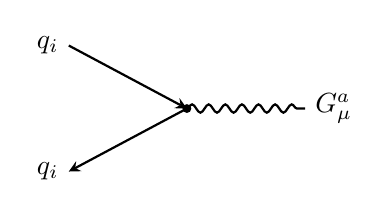
\begin{tikzpicture}[>=stealth]
  \coordinate (v) at (0,0);
  \draw[->,thick] (-1.5,0.8) node[left] {$q_i$} -- (v);
  \draw[->,thick] (v) -- (-1.5,-0.8) node[left] {$q_i$};
  \draw[decorate,decoration={snake,amplitude=1.5pt,segment length=6pt},thick]
    (v) -- (1.5,0) node[right] {$G_\mu^a$};
  \fill (v) circle (1.6pt);
\end{tikzpicture}
\hspace{1.2cm}
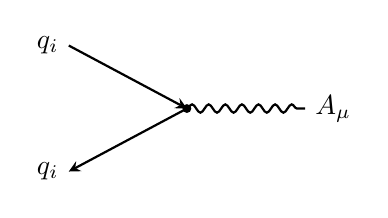
\begin{tikzpicture}[>=stealth]
  \coordinate (v) at (0,0);
  \draw[->,thick] (-1.5,0.8) node[left] {$q_i$} -- (v);
  \draw[->,thick] (v) -- (-1.5,-0.8) node[left] {$q_i$};
  \draw[decorate,decoration={snake,amplitude=1.5pt,segment length=6pt},thick]
    (v) -- (1.5,0) node[right] {$A_\mu$};
  \fill (v) circle (1.6pt);
\end{tikzpicture}
\caption{The two gauge interactions of a quark in $SU(3)_c\times U(1)_{\mathrm{EM}}$. The gluon vertex carries the color generator $\lambda^a/2$, while the photon vertex carries the electric charge $Q_f$.}
\label{fig:lec15:qcd-qed-quark-vertices}
\end{figure}

In the mass basis the quark mass terms are
\begin{equation}
  \boxed{\;
  \Lag_{\mathrm{mass}}^{q}
  =-m_u\bar uu-m_c\bar cc-m_t\bar tt
   -m_d\bar dd-m_s\bar ss-m_b\bar bb\; .}
  \label{eq:lec15:quark_mass_terms}
\end{equation}

\textit{Significance:} The mass eigenstates preserve electric charge: $u,c,t$ have $Q=+2/3$, while $d,s,b$ have $Q=-1/3$.

One may also add the three charged leptons $\ell_i=e,\mu,\tau$, which transform as
\begin{equation}
  \ell_{Li}\sim(\mathbf1,-1),\qquad \ell_{Ri}\sim(\mathbf1,-1).
  \label{eq:lec15:charged_lepton_representations}
\end{equation}
Since they are $SU(3)_c$ singlets, their covariant derivative contains only the electromagnetic term:
\begin{equation}
  D_\mu\ell_i=(\partial_\mu-i e A_\mu)\ell_i .
  \label{eq:lec15:lepton_covariant_derivative}
\end{equation}

\subsubsection*{Accidental Global Symmetries}

The gauge symmetry is imposed. The global symmetry is what remains accidentally after the allowed kinetic and mass terms are written. In pure $\QCD$ the kinetic terms treat all six quark flavors alike, giving $U(6)_L\times U(6)_R$. Once electromagnetism is included, the up-type and down-type sectors have different $U(1)_{\mathrm{EM}}$ charges, so they cannot be rotated into one another without changing the photon coupling. The kinetic terms therefore have
\begin{equation}
  \boxed{\;G_{\mathrm{global,kin}}
  =U(3)_{u_L}\times U(3)_{u_R}\times U(3)_{d_L}\times U(3)_{d_R}\; .}
  \label{eq:lec15:qcd_qed_kinetic_global_symmetry}
\end{equation}

\textit{Significance:} Electromagnetism reduces the accidental flavor symmetry because electric charge distinguishes the two quark sectors.

After diagonal mass terms are included, the independent non-Abelian rotations are broken. If all six masses are nondegenerate, the surviving quark flavor symmetries are the six separate phase rotations
\begin{equation}
  \boxed{\;G_{\mathrm{global,full}}=U(1)_u\times U(1)_c\times U(1)_t
  \times U(1)_d\times U(1)_s\times U(1)_b\simeq U(1)^6\; .}
  \label{eq:lec15:qcd_qed_full_global_symmetry}
\end{equation}

\textit{Significance:} In the absence of weak interactions, each quark flavor number is separately conserved.

%%==================================================================
\subsection{What Spontaneous Symmetry Breaking Means}\label{subsec:lec15:ssb-meaning}

\subsubsection*{Conceptual Background}

A symmetry of the Lagrangian is a symmetry of the equations of motion and of the full theory. A vacuum is a particular lowest-energy configuration around which perturbation theory is performed. Spontaneous symmetry breaking occurs when the Lagrangian is invariant under a symmetry, but the chosen vacuum is not invariant under that symmetry.

\dfn[def:lec15:ssb]{Spontaneous Symmetry Breaking}{
A symmetry transformation $g$ is spontaneously broken if
\begin{equation}
  \Lag[g\phi]=\Lag[\phi],
  \qquad
  g\langle\phi\rangle\neq \langle\phi\rangle .
  \label{eq:lec15:ssb_definition}
\end{equation}
Here $\langle\phi\rangle$ denotes the vacuum expectation value, namely the field value in the chosen vacuum.
}

The reason this matters phenomenologically is that perturbative particles are excitations around the vacuum. If the vacuum is not symmetric, the Lagrangian written in terms of the excitation fields need not display the original symmetry term by term, even though the underlying theory still knows about it through relations among couplings.

\nt{Spontaneous breaking is not the same as explicitly removing the symmetry. If the symmetry is explicit, the most general Lagrangian has more independent parameters. If the symmetry is spontaneous, the broken-phase Lagrangian can contain terms that look asymmetric, but their coefficients remain related by the symmetric parent theory.}

%%==================================================================
\subsection{\texorpdfstring{Discrete Example: A Real Scalar with $\mathbb Z_2$}{Discrete Example: A Real Scalar with Z2}}\label{subsec:lec15:z2-real-scalar}

\subsubsection*{Physical Motivation}

The simplest example uses one real scalar field $\phi(x)$ and the discrete symmetry
\begin{equation}
  \mathbb Z_2:\qquad \phi\to-\phi .
  \label{eq:lec15:z2_transformation}
\end{equation}
Because odd powers change sign, the symmetry forbids terms such as $\phi$ and $\phi^3$.

\subsubsection*{Mathematical Setup}

The most general renormalizable Lagrangian with this symmetry is
\begin{equation}
  \boxed{\;\Lag
  =\frac12\partial_\mu\phi\,\partial^\mu\phi
   -\frac12\mu^2\phi^2
   -\frac{\lambda}{4}\phi^4\; ,\qquad \lambda>0\; .}
  \label{eq:lec15:z2_lagrangian}
\end{equation}

\textit{Significance:} The sign of $\mu^2$ decides whether the symmetry is visible in the vacuum or hidden by the vacuum choice.

The potential energy is
\begin{equation}
  V(\phi)=\frac12\mu^2\phi^2+\frac{\lambda}{4}\phi^4 .
  \label{eq:lec15:z2_potential}
\end{equation}
The extrema solve
\begin{align}
  0=\frac{dV}{d\phi}
  &=\mu^2\phi+\lambda\phi^3
    =\phi(\mu^2+\lambda\phi^2).
  \label{eq:lec15:z2_stationary_condition}
\end{align}
There are two cases.

\paragraph{Unbroken case: $\mu^2>0$.}
The only real stationary point is $\phi=0$. The second derivative is
\begin{equation}
  \frac{d^2V}{d\phi^2}\bigg|_{\phi=0}=\mu^2>0,
  \label{eq:lec15:z2_unbroken_second_derivative}
\end{equation}
so $\phi=0$ is the vacuum. Since $\phi=0$ is unchanged by $\phi\to-\phi$, the vacuum respects $\mathbb Z_2$.

\paragraph{Broken case: $\mu^2<0$.}
The nonzero stationary points satisfy
\begin{equation}
  \phi^2=-\frac{\mu^2}{\lambda}\equiv v^2,
  \qquad
  v=\sqrt{-\frac{\mu^2}{\lambda}} .
  \label{eq:lec15:z2_v_definition}
\end{equation}
At these points
\begin{equation}
  \frac{d^2V}{d\phi^2}\bigg|_{\phi=\pm v}
  =\mu^2+3\lambda v^2
  =\mu^2+3\lambda\left(-\frac{\mu^2}{\lambda}\right)
  =-2\mu^2
  =2\lambda v^2>0,
  \label{eq:lec15:z2_broken_second_derivative}
\end{equation}
so the two classical minima are
\begin{equation}
  \boxed{\;\langle\phi\rangle=+v\quad\text{or}\quad \langle\phi\rangle=-v\; .}
  \label{eq:lec15:z2_two_vacua}
\end{equation}

\textit{Significance:} The two vacua are physically equivalent, but either single choice is not invariant under $\phi\to-\phi$.

\begin{figure}[ht]
\centering
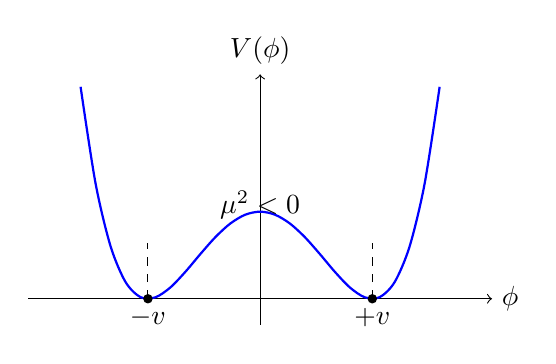
\begin{tikzpicture}[scale=0.95]
  \draw[->] (-3.1,0) -- (3.1,0) node[right] {$\phi$};
  \draw[->] (0,-0.35) -- (0,3.0) node[above] {$V(\phi)$};
  \draw[domain=-2.4:2.4,smooth,variable=\x,thick,blue]
    plot ({\x},{0.23*(\x*\x-2.25)^2});
  \fill (-1.5,0) circle (1.8pt) node[below] {$-v$};
  \fill (1.5,0) circle (1.8pt) node[below] {$+v$};
  \node at (0,1.25) {$\mu^2<0$};
  \draw[dashed] (-1.5,0) -- (-1.5,0.75);
  \draw[dashed] (1.5,0) -- (1.5,0.75);
\end{tikzpicture}
\caption{The $\mathbb Z_2$-symmetric potential for $\mu^2<0$. The Lagrangian is symmetric under reflection $\phi\to-\phi$, but choosing either minimum selects one side.}
\label{fig:lec15:z2-double-well}
\end{figure}

\subsubsection*{Expansion around the Vacuum}

Choose, without loss of generality, the vacuum $+v$. Define the excitation field
\begin{equation}
  \phi(x)=v+\phi'(x),
  \qquad
  \langle\phi'\rangle=0 .
  \label{eq:lec15:z2_shift}
\end{equation}
The kinetic term is unchanged because $v$ is constant:
\begin{equation}
  \partial_\mu\phi=\partial_\mu\phi' .
  \label{eq:lec15:z2_kinetic_shift}
\end{equation}
The potential becomes
\begin{align}
  V(v+\phi')
  &=\frac12\mu^2(v+\phi')^2+\frac{\lambda}{4}(v+\phi')^4
    \notag\\
  &=\frac12\mu^2(v^2+2v\phi'+\phi'^2)
    +\frac{\lambda}{4}
      \left(v^4+4v^3\phi'+6v^2\phi'^2+4v\phi'^3+\phi'^4\right)
    \notag\\
  &=\left(\frac12\mu^2v^2+\frac{\lambda}{4}v^4\right)
    +(\mu^2v+\lambda v^3)\phi'
    +\left(\frac12\mu^2+\frac32\lambda v^2\right)\phi'^2
    +\lambda v\phi'^3+\frac{\lambda}{4}\phi'^4 .
  \label{eq:lec15:z2_potential_expansion}
\end{align}
Using the minimum condition $\mu^2+\lambda v^2=0$, the linear term vanishes and
\begin{equation}
  \frac12\mu^2+\frac32\lambda v^2
  =-\frac12\lambda v^2+\frac32\lambda v^2
  =\lambda v^2 .
  \label{eq:lec15:z2_quadratic_coefficient}
\end{equation}
Dropping the irrelevant constant vacuum energy, the Lagrangian in terms of the physical excitation is
\begin{equation}
  \boxed{\;\Lag
  =\frac12\partial_\mu\phi'\,\partial^\mu\phi'
   -\frac12(2\lambda v^2)\phi'^2
   -\lambda v\phi'^3
   -\frac{\lambda}{4}\phi'^4\; .}
  \label{eq:lec15:z2_shifted_lagrangian}
\end{equation}

\textit{Significance:} The broken-phase Lagrangian contains a cubic interaction, but its coefficient is fixed by the same two parameters that controlled the original symmetric theory.

Comparing the quadratic term to $-\frac12m_{\phi'}^2\phi'^2$ gives
\begin{equation}
  \boxed{\;m_{\phi'}^2=2\lambda v^2=-2\mu^2>0\; .}
  \label{eq:lec15:z2_scalar_mass}
\end{equation}

\textit{Significance:} A negative $\mu^2$ in the symmetric-field coordinates is not a physical negative mass squared after expanding around the true vacuum.

\begin{figure}[ht]
\centering
\begin{tikzpicture}
  \coordinate (v) at (0,0);
  \foreach \ang in {90,210,330} {
    \draw[thick] (v) -- (\ang:1.2);
  }
  \node at (90:1.38) {$\phi'$};
  \node at (210:1.38) {$\phi'$};
  \node at (330:1.38) {$\phi'$};
  \fill (v) circle (1.6pt);
\end{tikzpicture}
\hspace{1.2cm}
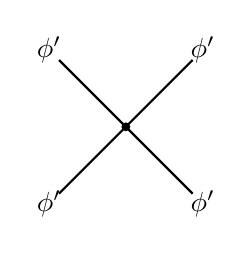
\begin{tikzpicture}
  \coordinate (v) at (0,0);
  \foreach \ang in {45,135,225,315} {
    \draw[thick] (v) -- (\ang:1.2);
  }
  \node at (45:1.38) {$\phi'$};
  \node at (135:1.38) {$\phi'$};
  \node at (225:1.38) {$\phi'$};
  \node at (315:1.38) {$\phi'$};
  \fill (v) circle (1.6pt);
\end{tikzpicture}
\caption{Scalar self-interactions after $\mathbb Z_2$ spontaneous symmetry breaking. The cubic vertex appears only after shifting to the vacuum, and its coefficient is related to the quartic coupling and $v$.}
\label{fig:lec15:z2-broken-scalar-vertices}
\end{figure}

\clm[clm:lec15:ssb-parameter-counting]{Parameter Counting after Spontaneous Breaking}{
Spontaneous symmetry breaking changes the variables used to describe the theory, but it does not introduce new independent parameters. In the $\mathbb Z_2$ example, the broken-phase coefficients $m_{\phi'}^2$, $\lambda v$, and $\lambda$ are all functions of the original two quantities $\mu^2$ and $\lambda$.
}

For renormalizable scalar terms in four spacetime dimensions, the coefficients with positive mass dimension can change after shifting by the vacuum, while the dimensionless quartic coupling remains the same. The lecture emphasized this because relations among broken-phase parameters are what make spontaneously broken theories predictive.

%%==================================================================
\subsection{\texorpdfstring{Continuous Example: Global $U(1)$}{Continuous Example: Global U(1)}}\label{subsec:lec15:global-u1}

\subsubsection*{Physical Motivation}

A continuous symmetry has a qualitatively new feature: if the vacuum manifold is continuous, one can move along it without changing the potential energy. That flat direction becomes a massless particle in the quantum theory.

Take one complex scalar field $\phi$ with global $U(1)$ charge $+1$:
\begin{equation}
  U(1):\qquad \phi\to e^{i\theta}\phi ,
  \label{eq:lec15:u1_transformation}
\end{equation}
where $\theta$ is a constant real angle.

\subsubsection*{Mathematical Setup}

The renormalizable $U(1)$-invariant Lagrangian is
\begin{equation}
  \boxed{\;\Lag
  =\partial_\mu\phi^\dagger\partial^\mu\phi
   -\mu^2\phi^\dagger\phi
   -\lambda(\phi^\dagger\phi)^2\; ,\qquad \lambda>0\; .}
  \label{eq:lec15:u1_lagrangian_complex}
\end{equation}

\textit{Significance:} The potential depends only on the magnitude of $\phi$, so a nonzero vacuum will have a continuous degeneracy of phases.

It is often useful to write the complex field in terms of two real fields $h$ and $\chi$:
\begin{equation}
  \phi=\frac{1}{\sqrt2}(h+i\chi),
  \qquad
  \phi^\dagger\phi=\frac12(h^2+\chi^2).
  \label{eq:lec15:u1_real_components}
\end{equation}
In this language the same symmetry is an $SO(2)$ rotation:
\begin{equation}
  \begin{pmatrix}h\\ \chi\end{pmatrix}
  \to
  \begin{pmatrix}
    \cos\theta & \sin\theta\\
    -\sin\theta & \cos\theta
  \end{pmatrix}
  \begin{pmatrix}h\\ \chi\end{pmatrix}.
  \label{eq:lec15:u1_so2_rotation}
\end{equation}
Substituting Eq.~\eqref{eq:lec15:u1_real_components} into Eq.~\eqref{eq:lec15:u1_lagrangian_complex} gives
\begin{equation}
  \boxed{\;\Lag
  =\frac12\partial_\mu h\,\partial^\mu h
   +\frac12\partial_\mu\chi\,\partial^\mu\chi
   -\frac{\mu^2}{2}(h^2+\chi^2)
   -\frac{\lambda}{4}(h^2+\chi^2)^2\; .}
  \label{eq:lec15:u1_lagrangian_real}
\end{equation}

\textit{Significance:} Before choosing a vacuum, the two real fields are indistinguishable directions in the same symmetric plane.

For $\mu^2<0$, define
\begin{equation}
  v^2\equiv-\frac{\mu^2}{\lambda}>0 .
  \label{eq:lec15:u1_v_definition}
\end{equation}
The potential can be written, up to an additive constant, as
\begin{equation}
  \boxed{\;V(\phi)=\lambda\left(\phi^\dagger\phi-\frac{v^2}{2}\right)^2\; .}
  \label{eq:lec15:u1_mexican_hat_potential}
\end{equation}

\textit{Significance:} The vacuum condition fixes only the radius in field space, not the angular direction.

The minimum condition is
\begin{equation}
  \phi^\dagger\phi=\frac{v^2}{2}
  \qquad\Longleftrightarrow\qquad
  h^2+\chi^2=v^2 .
  \label{eq:lec15:u1_vacuum_manifold}
\end{equation}
Thus the set of vacua is a circle of radius $v$ in the $(h,\chi)$ plane.

\begin{figure}[ht]
\centering
\begin{tikzpicture}[scale=0.95]
  \draw[->] (-2.7,0) -- (2.7,0) node[right] {$h$};
  \draw[->] (0,-2.2) -- (0,2.2) node[above] {$\chi$};
  \draw[thick,blue] (0,0) circle (1.35);
  \fill (1.35,0) circle (2pt) node[below right] {chosen vacuum};
  \draw[->,red,thick] (1.35,0) -- (2.25,0) node[right] {massive radial mode $h'$};
  \draw[->,myg,thick] (1.35,0) arc[start angle=0,end angle=38,radius=1.35]
    node[above right] {massless angular mode $\chi'$};
  \node at (-1.7,1.65) {$h^2+\chi^2=v^2$};
\end{tikzpicture}
\caption{The vacuum manifold of the broken global $U(1)$ theory. Motion radially changes the potential and gives a massive excitation; motion tangentially stays on the degenerate circle and gives a Goldstone boson.}
\label{fig:lec15:u1-vacuum-circle}
\end{figure}

\subsubsection*{Expansion around a Chosen Vacuum}

Choose the vacuum in the positive real direction:
\begin{equation}
  \langle h\rangle=v,\qquad \langle\chi\rangle=0 .
  \label{eq:lec15:u1_chosen_vacuum}
\end{equation}
Define fluctuation fields with zero vacuum expectation values:
\begin{equation}
  h=v+h',
  \qquad
  \chi=\chi',
  \qquad
  \langle h'\rangle=\langle\chi'\rangle=0.
  \label{eq:lec15:u1_shift}
\end{equation}
Now
\begin{align}
  h^2+\chi^2
  &=(v+h')^2+\chi'^2
   =v^2+2vh'+h'^2+\chi'^2,
  \label{eq:lec15:u1_radius_shift}\\
  h^2+\chi^2-v^2
  &=2vh'+h'^2+\chi'^2 .
  \label{eq:lec15:u1_radius_minus_v}
\end{align}
Using
\[
  V=\frac{\lambda}{4}(h^2+\chi^2-v^2)^2,
\]
we get
\begin{align}
  V
  &=\frac{\lambda}{4}
    \left(2vh'+h'^2+\chi'^2\right)^2
    \notag\\
  &=\frac{\lambda}{4}
    \left[
      4v^2h'^2
      +4vh'(h'^2+\chi'^2)
      +(h'^2+\chi'^2)^2
    \right]
    \notag\\
  &=\lambda v^2h'^2
    +\lambda vh'(h'^2+\chi'^2)
    +\frac{\lambda}{4}(h'^2+\chi'^2)^2 .
  \label{eq:lec15:u1_potential_expansion}
\end{align}
The broken-phase Lagrangian is therefore
\begin{equation}
  \boxed{\;\Lag
  =\frac12\partial_\mu h'\partial^\mu h'
   +\frac12\partial_\mu\chi'\partial^\mu\chi'
   -\lambda v^2h'^2
   -\lambda vh'(h'^2+\chi'^2)
   -\frac{\lambda}{4}(h'^2+\chi'^2)^2\; .}
  \label{eq:lec15:u1_shifted_lagrangian}
\end{equation}

\textit{Significance:} The original $SO(2)$ rotation symmetry is hidden in the shifted variables, but it still enforces the precise pattern of masses and interactions.

Reading off the quadratic terms gives
\begin{equation}
  \boxed{\;m_{h'}^2=2\lambda v^2=-2\mu^2,\qquad m_{\chi'}^2=0\; .}
  \label{eq:lec15:u1_masses}
\end{equation}

\textit{Significance:} The radial excitation is massive, while the angular excitation is massless because changing the phase moves along a degenerate set of vacua.

\begin{figure}[ht]
\centering
\begin{tikzpicture}
  \coordinate (v) at (0,0);
  \draw[thick] (-1.0,0.8) node[left] {$\chi'$} -- (v);
  \draw[thick] (-1.0,-0.8) node[left] {$\chi'$} -- (v);
  \draw[thick] (v) -- (1.3,0) node[right] {$h'$};
  \fill (v) circle (1.6pt);
\end{tikzpicture}
\hspace{1.0cm}
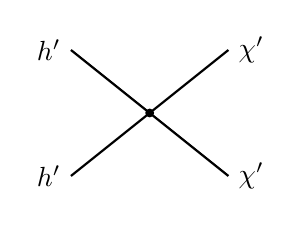
\begin{tikzpicture}
  \coordinate (v) at (0,0);
  \draw[thick] (-1.0,0.8) node[left] {$h'$} -- (v);
  \draw[thick] (-1.0,-0.8) node[left] {$h'$} -- (v);
  \draw[thick] (1.0,0.8) node[right] {$\chi'$} -- (v);
  \draw[thick] (1.0,-0.8) node[right] {$\chi'$} -- (v);
  \fill (v) circle (1.6pt);
\end{tikzpicture}
\caption{Representative broken-phase scalar interactions in the global $U(1)$ model. The $h'\chi'\chi'$ and $h'h'\chi'\chi'$ interactions are not arbitrary; they are fixed by the same $\lambda$ and $v$ that determine the radial mass.}
\label{fig:lec15:u1-broken-scalar-vertices}
\end{figure}

\clm[clm:lec15:different-vacuum-same-physics]{Choice of Vacuum Does Not Change the Physics}{
Choosing a different point on the circle $h^2+\chi^2=v^2$ merely rotates which linear combination of the original fields is called the radial mode and which is called the angular mode. The spectrum still contains one scalar of mass squared $2\lambda v^2$ and one massless scalar.
}

%%==================================================================
\subsection{Tachyons and the Meaning of Negative Mass Squared}\label{subsec:lec15:tachyons}

\subsubsection*{Conceptual Background}

In the original symmetric coordinates, the parameter choice $\mu^2<0$ makes the quadratic term look like a negative mass squared around $\phi=0$. A particle with negative mass squared is often called a tachyon. In this context, however, the tachyon is not a physical asymptotic particle; it is a warning that $\phi=0$ is not the correct vacuum.

\dfn[def:lec15:tachyon]{Tachyon in a Scalar Potential}{
A tachyonic quadratic term means that the curvature of the potential at the expansion point is negative:
\begin{equation}
  \boxed{\;m_{\mathrm{local}}^2
  =\frac{d^2V}{d\phi^2}\bigg|_{\mathrm{expansion\ point}}<0\; .}
  \label{eq:lec15:tachyonic_curvature}
\end{equation}
}

\textit{Significance:} A tachyonic mass parameter signals an unstable expansion point, not a stable faster-than-light particle in the physical spectrum.

At the true minimum in the $\mathbb Z_2$ example, the curvature is instead
\begin{equation}
  \frac{d^2V}{d\phi^2}\bigg|_{\phi=\pm v}=2\lambda v^2>0,
  \label{eq:lec15:true_vacuum_positive_curvature}
\end{equation}
so the excitation field $\phi'$ has an ordinary positive mass squared. This is why perturbative $\QFT$ is built around minima of the potential: physical particles are small oscillations around a stable ground state.

%%==================================================================
\subsection{Goldstone Bosons}\label{subsec:lec15:goldstone}

\subsubsection*{Physical Motivation}

In the global $U(1)$ example, the vacuum manifold is a circle. Once a point on the circle is chosen, there are two qualitatively different infinitesimal motions:
\begin{itemize}
  \item moving radially changes $h^2+\chi^2$ and therefore changes the potential energy;
  \item moving tangentially along the circle keeps $h^2+\chi^2=v^2$ and therefore costs no potential energy.
\end{itemize}
The second motion is a flat direction, and a flat direction has zero restoring force. Since mass squared is the curvature of the potential, zero curvature means a massless scalar.

\thm[thm:lec15:goldstone-theorem]{Goldstone Theorem}{
For every spontaneously broken continuous global symmetry generator, the theory contains a massless boson, called a Goldstone boson.
\begin{equation}
  \boxed{\;N_{\mathrm{Goldstone}}
  =N_{\mathrm{broken\ continuous\ global\ generators}}\; .}
  \label{eq:lec15:goldstone_counting}
\end{equation}
}

\textit{Significance:} Massless scalars are not accidental details of the example; they are forced by the geometry of a continuously degenerate vacuum.

For the global $U(1)$ model, there is one generator and it is broken by choosing $\langle\phi\rangle=v/\sqrt2$. Therefore Eq.~\eqref{eq:lec15:goldstone_counting} predicts one Goldstone boson, precisely the field $\chi'$ found in Eq.~\eqref{eq:lec15:u1_masses}. In later lectures, gauging the symmetry will modify this conclusion and lead to the Higgs mechanism.
